\section{Andersen Thermostat}

The Andersen thermostat is an easier model than the Langevin thermostat. 
As before we assume a solvent but now there is no friction but only random velocity replacement. 
We simply state, that a particle gets a normal distributed velocity through collisions with the solvent with a certain probability. 
The mean difference is that we are are not assuming a random \textbf{force} but a new random \textbf{velocity}, no matter which velocity the particle had before.
This is not physical!\\

Due to this the Andersen thermostat creates a (N,V,T)-ensemble, but not allows to determine dynamical properties of the system, because the random velocity replacement destroys the memory of the system (especially if there is only one particle or no interaction between particles).

\subsection{Implementation}

For the Andersen thermostat most parts of the existing script can be used.
The new part is the function step\_vv\_andersen() which you can see in code block \ref{andersen}.

\listfile{../src/ljsim.py}{src/ljsim.py}{115}{138}{Andersen thermostat}{andersen}

The function equals the original step\_vv() function except that there is the velocity replacement at the end.
In line 141 it loops over all particles.
This may not be necessary when simulating only one particle, but it allows to use other initial conditions for the same script with more than one particle.
The next line asks weather a random number is smaller than $\nu \D t$ where --nu allows you to pass a parameter nu (default: $\nu =0.1$).
This term represents the probability for a stochastic collision.
If the statement is fulfilled the velocity of the selected particle is replaced by a normal distributed random velocity with a deviation of $\sigma =\sqrt{T_\text{des}}$.

\subsection{Simulation}

Simulating with the Andersen thermostat works exactly like in the former task.
The results can be seen in the figures \ref{andersenT} and \ref{andersenvv}.

\begin{figure}[ht]
	\centering
	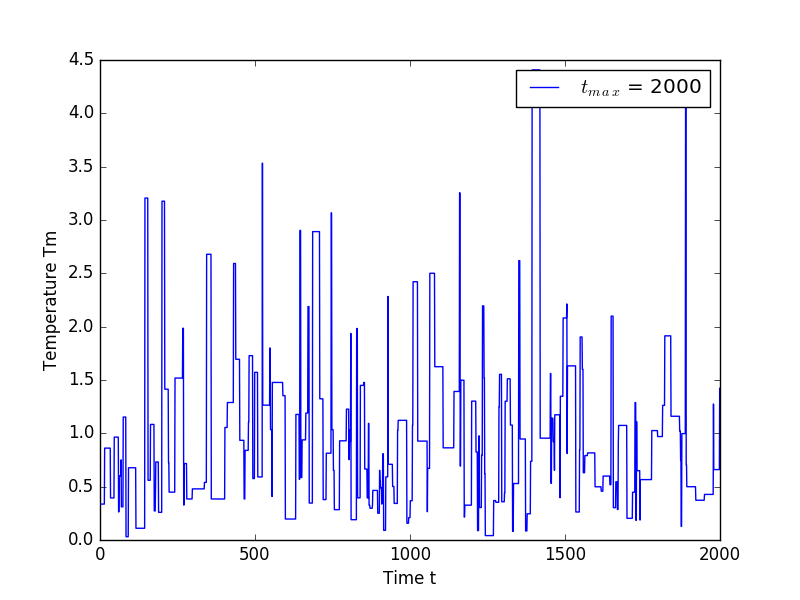
\includegraphics[width=0.7\textwidth]{../dat/andersen_T1d0_nu0d1_Tm.png}
	\caption{
		Plot of the temperature over time for a desired temperature of $T_\text{des}=1.0$ for a simulation with the Andersen thermostat and $\nu =0.3$.
	}
	\label{andersenT}
\end{figure}

\begin{figure}[ht]
	\centering
	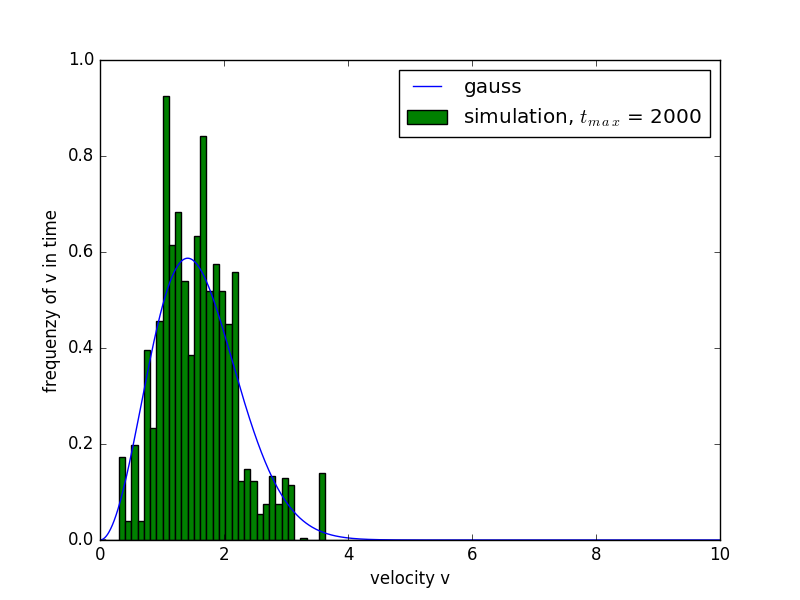
\includegraphics[width=0.7\textwidth]{../dat/andersen_T1d0_nu0d1_vv.png}
	\caption{
		Plot of the temperature over time for a desired temperature of $T_\text{des}=1.0$ for a simulation with the Andersen thermostat and $\nu =0.3$.
	}
	\label{andersenvv}
\end{figure}

As you can see the temperature is also varying around 1.0 but not with the same regularity. 
The velocity distribution comes near to the Gaussian but it does not fit as good as for the Langevin thermostat.

\FloatBarrier 
